\section{Related Work}

\begin{figure*}[t]
    \centering
    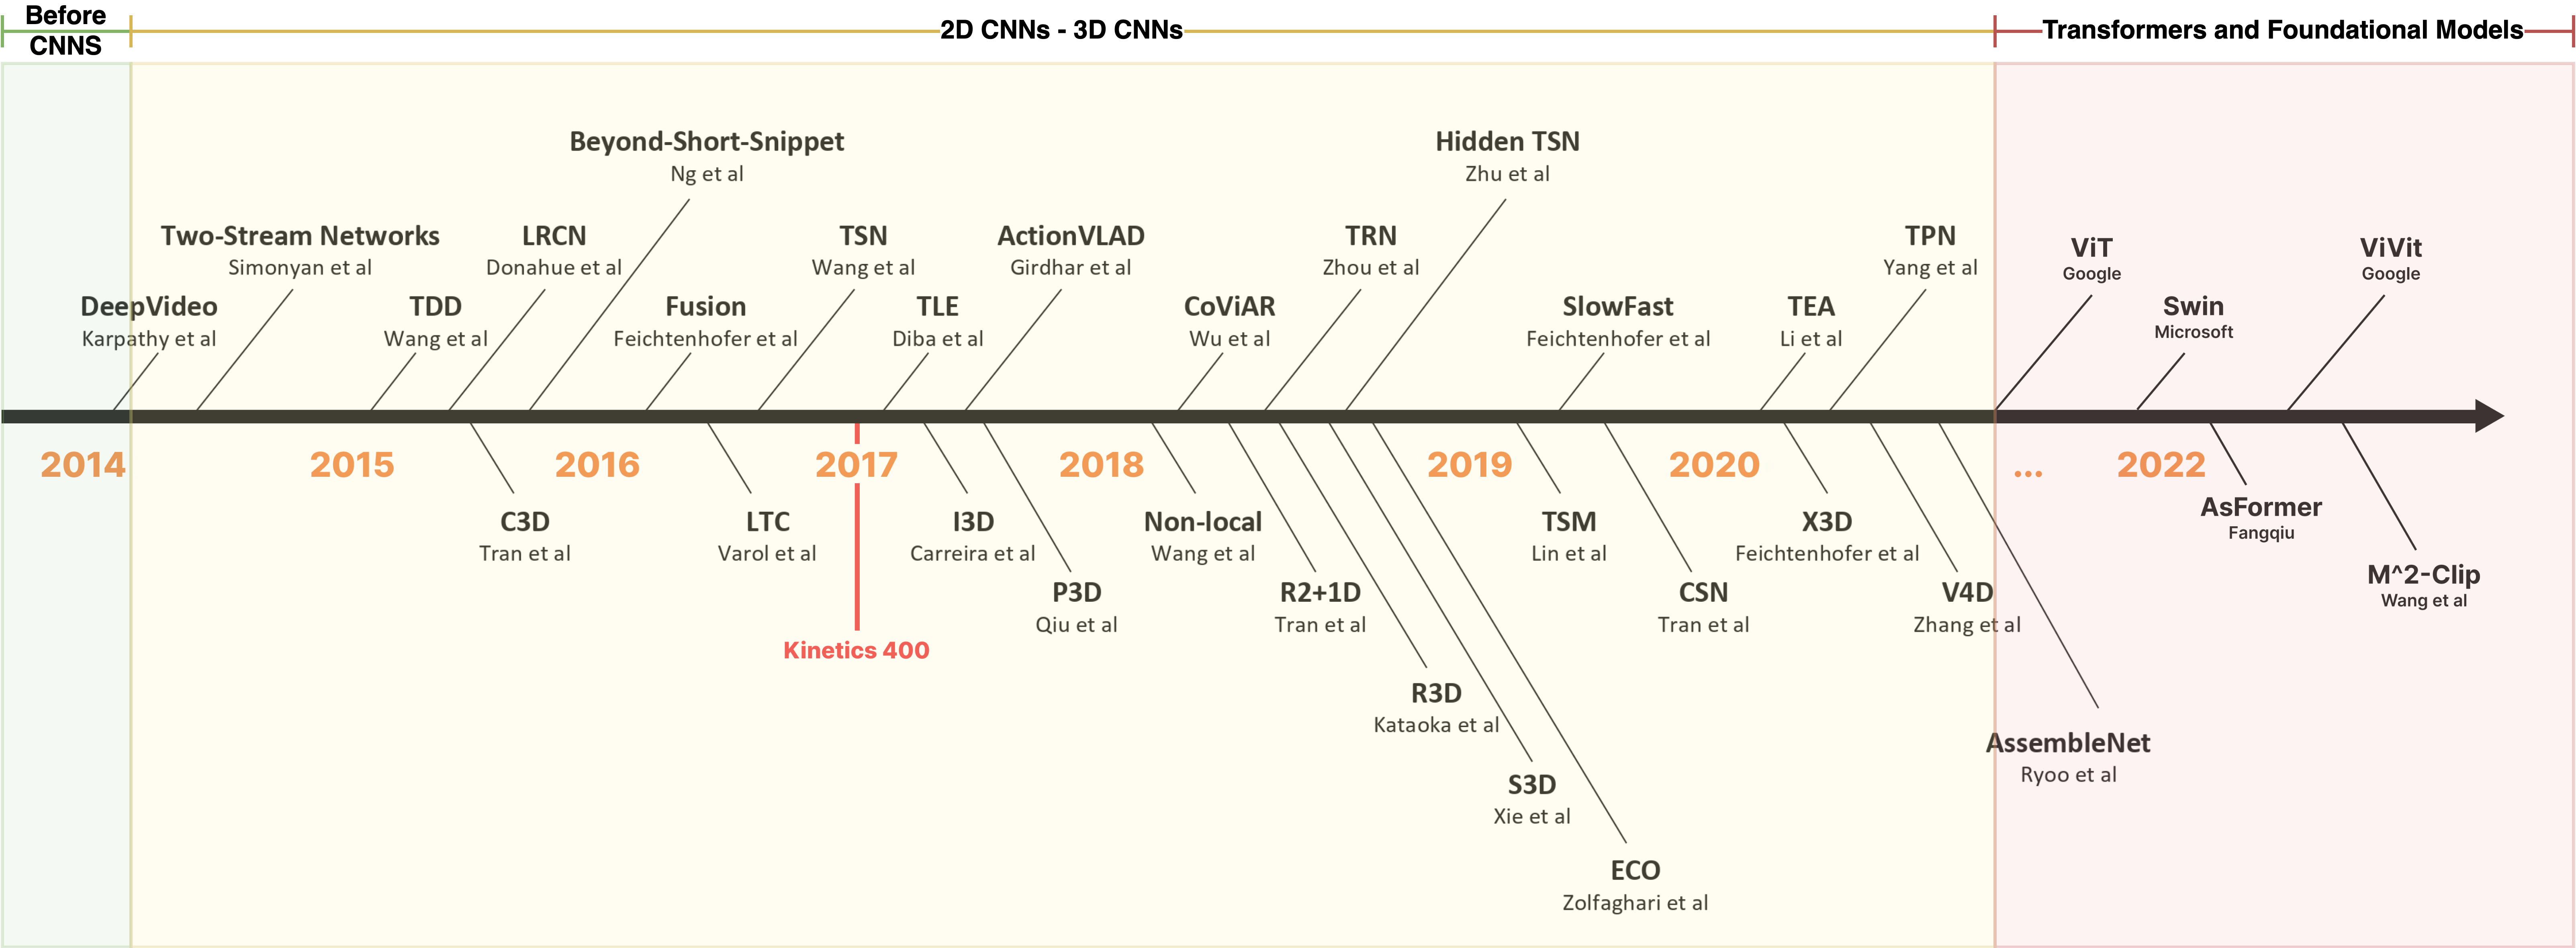
\includegraphics[width=\textwidth]{../../assets/figures/extended-video-timeline-v3.png}
    \caption{A timeline overview of the evolution of video analysis models.}
    \label{figure:video-models-evolution}
    \cite{video-action-recognition-study}
\end{figure*}

In this section, we explore some of the prominent approaches to temporal action segmentation (TAS), discussing how methods have evolved over time as computational power and dataset availability have increased.

\subsection{The Evolution of Video Analysis Models}

The development of video analysis models has seen a significant shift as computational power and dataset size have increased. Initially, video analysis relied heavily on hand-crafted feature extraction \cite{handcrafted-features-1,handcrafted-features-2}, where specific features such as pixels were manually chosen or extracted. With the introduction of optical flow\cite{i3d}, models began incorporating motion information, improving their ability to understand temporal sequences in videos.

As 2D Convolution Neural Networks (CNNs) gained popularity, they were applied to video data for feature extraction, showing promising results for action recognition \cite{tsn}. Following this, the introduction of 3D Temporal CNNs \cite{s3d,r3d,x3d,i3d,slowfast} allowed for better understanding of the temporal dimension in videos. These methods, combined with the advent of larger datasets like Kinetics \cite{kinetics-400-dataset} and Something-Something \cite{something-something-dataset}, marked a turning point in video action recognition, leveraging deep learning to handle complex temporal and spatial patterns in video data.

In recent years, transformers have also emerged as a promising approach for video analysis. Initially used for NLP tasks, transformers have demonstrated strong potential for video action recognition \cite{vivit,dinov2,action-clip}. However, unlike CNNs, transformers lack strong inductive biases \cite{vit}, such as locality and translation invariance, which CNNs excel at. This makes transformers more dependent on massive amounts of data to perform effectively.

The increasing availability of video datasets and computational resources has catalyzed these developments, enabling more sophisticated models. However, video models still face significant challenges due to the vast and diverse distribution of video data. This distribution causes models to drift more rapidly compared to other data types, which makes generalization across different datasets more difficult. Consequently, large datasets are essential for training video models, and pre-trained models often struggle to generalize beyond their original training sets. Moreover, networks with a large number of parameters are particularly prone to overfitting when trained on smaller datasets \cite{r3d-paper}.

\subsection{Temporal Action Segmentation and Its Approaches}

Temporal Action Segmentation can be approached in several ways. Here, we explore a few key perspectives \cite{tas-survey}:

\noindent\textbf{1. Video Classification.} In video classification, the focus is on assigning a single action label to an entire video or segment, typically using models such as 2D or 3D CNNs. This is the most popular perspective in the field, with well-established pre-trained networks available for various datasets. 

\noindent\textbf{2. Temporal Action Detection / Localization.} In this approach, the goal is to detect the temporal boundaries of actions within a video. This task is more challenging than video classification as it requires the model to identify both the start and end of actions while also classifying them.

\subsection{Challenges}

Video data presents a challenging problem due to its vast and diverse distribution, causing models to drift more rapidly compared to other data types. Consequently, handling video data often requires significantly larger datasets, yet available datasets remain limited compared to image and text data. While datasets such as Kinetics, Something-Something, and HowTo100M have advanced the field, video models are still more computationally expensive (Figure \ref{figure:video-models-evolution}), and networks with a large number of parameters are particularly prone to overfitting when trained on smaller datasets \cite{resnet-3d}.